Since this tutorial is centered at the desgin and implementation
of subdivision surfaces, a short non-theoretic introduction of 
subdivision surfaces is given in this section. We are going to 
focus on the various refinement schemes and the connectivity 
properties. A compelete review on subdisviions can be find at 
\cite{siggraph1998notes}.

A subdivision surface is the limit surface resulted from the
application of a subdivision algorithm to a control mesh
(Figure \ref{fig:teaser}). The subdivision algorithm  
recursively \emph{refine} (subdivide) the control mesh and 
\emph{modify} (smooth) the geometry. A subdivision 
algorithm can be characterized by a \emph{refinement operator} 
and a \emph{modification operator}. 

Refinement operators edit the connectivity
and create a uniformly refined mesh from the source mesh.
These operators can be classified acoording to the refinement
patterns. Figure \ref{RefSchemes} shows four major patterns employed
in subdivision algorithms. Examples are 
Catmull-Clark subdivision (PQQ) \cite{cc},
Loop subdivision (PTQ) \cite{loop}, 
Doo-Sabin subdivision (DQQ) \cite{ds}
and $\sqrt{3}$ subdivision \cite{sqrt3}.
Subdivisions may employ a combination of two patterns.
Examples are Stam QT subdivision \cite{sqt} and 
4-3 subdivision \cite{43} (PQQ and PTQ).

\begin{figure}
  \centering
  \psfrag{PQQ}[]{\scriptsize PQQ} 
  \psfrag{PTQ}[]{\scriptsize PTQ}
  \psfrag{DQQ}[]{\scriptsize DQQ} 
  \psfrag{Sqrt3}[]{\scriptsize $\sqrt{3}$} 
  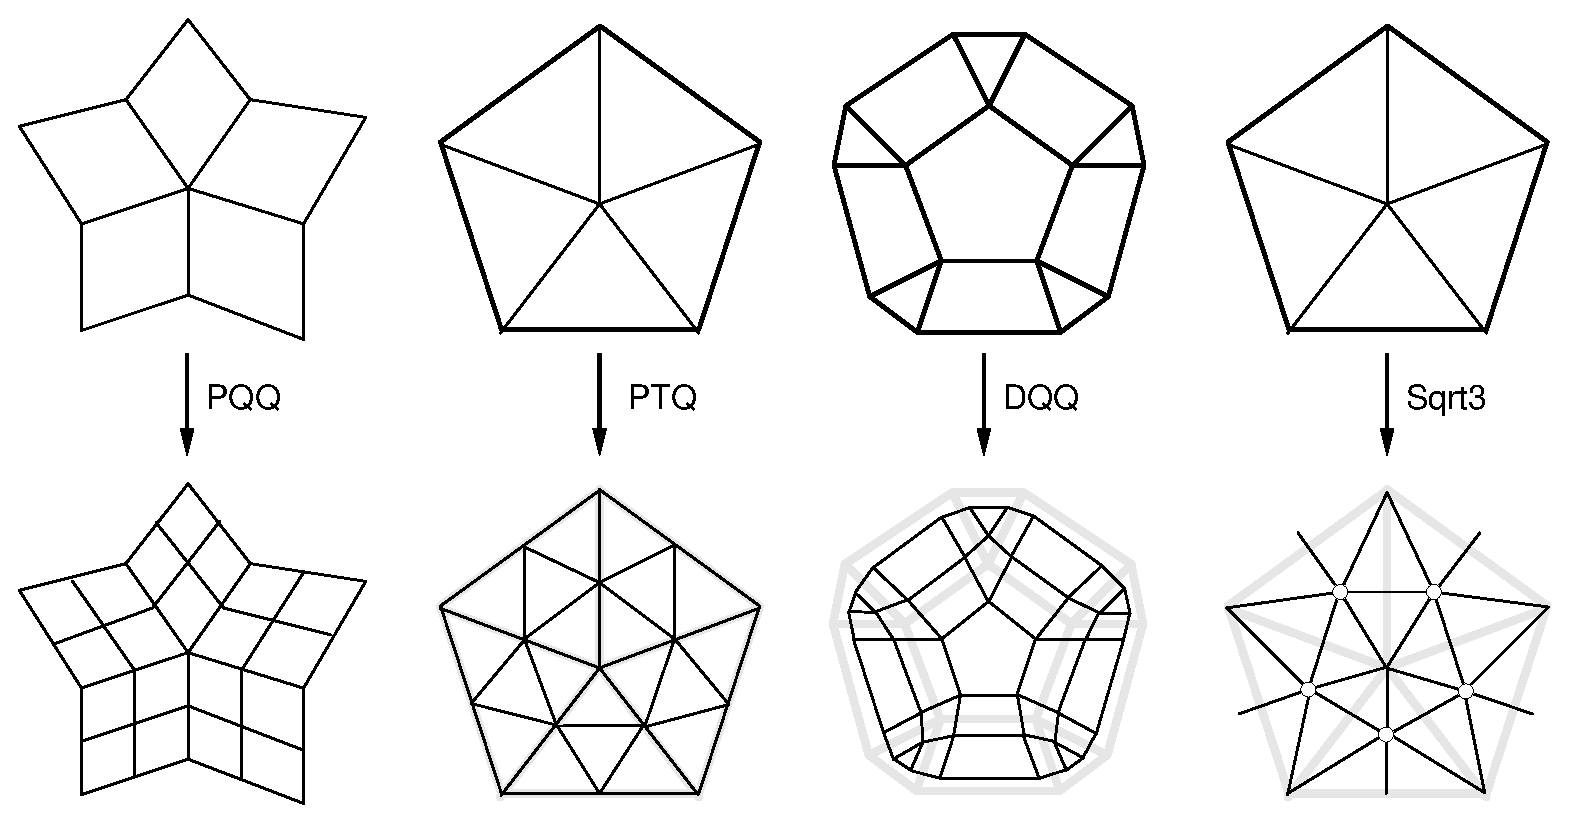
\epsfig{file=pfigs/RefSchemes.eps, width=4in}
  \caption{Refinement schemes: 
    primal quadrilateral quadrisection (PQQ),
    primal triangle quadrisection (PTQ),
    dual quadrilateral quadrisection (DQQ) and
    $\sqrt{3}$ refinement.}
  \label{fig:RefSchemes}
\end{figure}

Modification operators collect a submesh of the source
mesh and applied a stencil on the submesh to
generate the corresponding vertex of the refined mesh.
Figure \ref{fig:RefMap} demonstrates the examples of 
the correspondence between a source submesh and 
its target vertices.

\begin{figure}
  \centering
  \psfrag{A}[]{(a)}
  \psfrag{B}[]{(b)}
  \psfrag{C}[]{(c)}
  \psfrag{D}[]{(d)}
  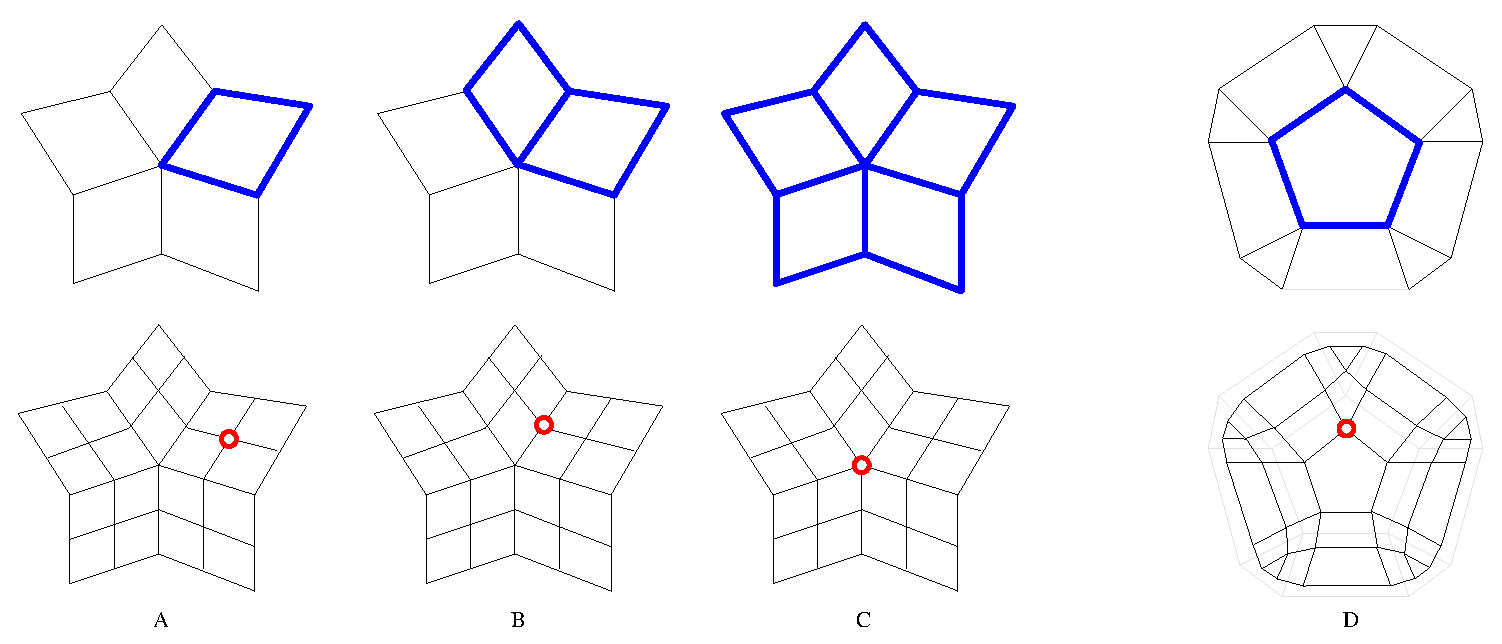
\epsfig{file=pfigs/RefMap.eps, width=4.5in}
  \caption{The correspondence of the source submesh and the 
           target vertex in the Catmull-Clark subdivision (a-c)
	   and Doo-Sabin subdivision (d). }
  \label{fig:RefMap}
\end{figure}

%% Any implementation of a subdivision scheme contains two major
%% components: \italic{refinement scheme} and \italic{geometry rules}.
%% Refinement schemes are defined by the 
%% \italic{uniform connectivity reconfiguration} of the source 
%% mesh (the domain) to the target mesh (the range). The geometry rules,
%% providing certain surface properties, e.g the smoothness, are the
%% mapping functions of the \italic{footprints} in the domain mesh to the
%% \italic{vertices} in the range mesh. Any subdivision in practice can
%% be defined as a legal combination of a refinement scheme and the
%% geometry rules. Based on the paradigm of the
%% \italic{policy-based design} \cite{a-rotm-02}, the combination can be
%% designed as the \italic{host function} (the refinement function)
%% templated with the \italic{policy class} (the geometry rules).
